\chapter{Fejlesztői dokumentáció}

Egy integrált fejlesztői környezetnél többféle igény is megfogalmazható. Valamelyik fejlesztőnek
olyanra van szüksége, amely ugyan kevesebbet tud, de gyorsabban indítható, esetlegesen gyorsabban
végezhető vele a munka. SQL-hez található több integrált fejlesztői környezet, ilyen az Oracle-nél
például az SQL Developer\cite{sqldeveloper}.
Az én programom az SQL Developerhez képest kevesebb komponenst tartalmaz, valamint nem Javaban, hanem C++ban lett írva,
így gyorsabb is. Tökéletes eszköz, ha valaki csak a lekérdezésekre próbál koncentrálni.

A megvalósított programban lehetőség van...
\begin{itemize}
  \item Oracle adatbázishoz való kapcsolódáshoz,
  \item kapcsolat adatainak mentésére,
  \item ezen kapcsolati adatok törlésére,
  \item PL/SQL szkriptek végrehajtására,
  \item SQL lekérdezések végrehajtására,
  \item adatbázis objektumok megtekintésére, törlésére,
  \item lekérdezési tervek létrehozására,
  \item kör, illetve oszlopdiagramok készítésére.
\end{itemize}

A fejlesztéshez szükséges eszközök kiválasztásnál tehát szempont volt a hatékonyság, valamint hogy
ennek ellenére többet nyújtson az eddig elérhető programoknál, ezért esett a választásom a Qt-ra, ami egy C++ keretrendszer.
Nem csak hatékony kódot lehet vele készíteni, szükség esetén magas absztrakció is használható, és nem
csak egy operációs rendszeren lehet a Qt-ban készített programokat futtatni. Ezen felül elvárás hogy legyen intuitív kezelőfelülete,
és biztonságosan működjön, ami a Qt objektum orientált felépítésének köszönhetően nagyon egyszerűen megoldható volt, és későbbi
bővítésekre is lehetőséget ad.

\section{Fogalmak}
Itt részleteznék néhány fogalmat amivel jobb tisztában lenni mielőtt tovább olvasná a dokumentációt.

Az SQL egy lekérdezésekre megfogalmazására specializálódott nyelv, azaz egy szakterület-specifikus nyelv.
PL/SQL az Oracle által az SQL kiterjesztéseként kifejlesztett procedurális programozási nyelv. Továbbá egy host nyelv,
amin belül bizonyos kódrészleteket SQL segítségével írhatunk meg. A C++ egy multi-paradigmás nyelv, így nem csak objektum orientáltan van lehetőség írni benne.
Így szokatlan lehet a legtöbb fejlesztő számára a funkcionális nyelv, amely paradigmából a névtelen függvény használatát vettem át. A névtelen függvény
egy helyben létrehozott, és akár meghívott függvény, amely jelentősen javíthat a kód olvashatóságán.

\section{Megoldási terv}

\begin{figure}[ht]
  \begin{center}
  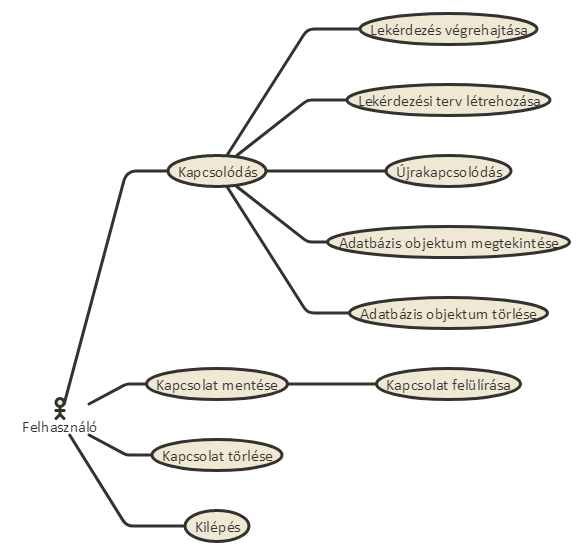
\includegraphics[scale=0.6]{usecase}
  \end{center}
 \caption{Felhasználói esetek}
\end{figure}

A felhasználóknak ezen felül lehetősége nyílhat más funkciók használatára is,
azonban ezek a legfontosabbak, így ezeknek az implementálása az elsődleges, ezért két külön ablakban történt a gyorsabb elérhetőség, és
a modularitás miatt. Ezáltal bármikor lehetőség nyílik új ablak nyitására, esetleg
ha valaki akar, akkor kódbol is csatlakozhat az adatbázishoz a forráskód birtokában.
Biztonsági szempontból ez nem ajánlatos, de ez is egy lehetőség ha nincs a számítógépen
biztonsági kockázat (pl. belső hálózatról működik csak, illetéktelen felhasználó nem férhet hozzá).

\subsection{Felhasználói felület terve}
\begin{figure}[ht]
  \begin{center}
  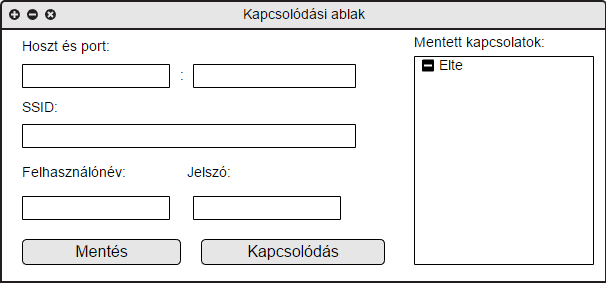
\includegraphics[scale=0.5]{connectionWindow}
  \end{center}
 \caption{Kapcsolódási ablak terve}
\end{figure}

A kapcsolódási ablaknál szempont volt az egyszerűség és könnyen kezelhetőség. Első használat
során már el lehet igazodni rajta bárkinek. Implementálás során fontos megjegyezni néhány szempontot
amit érdemes figyelmbe venni: a tabok sorrendje legyen meghatározott - balról jobbra, fentről lefele haladjon -, valamint
a jelszó mező tartalmát ne lehessen látni. Továbbá adatbázishoz kapcsolódás esetén legyen minél hamarabb eltűntetve a
jelszó a memóriából. (Megjegyzés: C++ esetén vigyázni kell az optimalizálásra, fordítótol függően könnyen lehet hogy a nem használt értékadást
eltűnteti a fordító) A kapcsolatokat lehessen szerkeszteni, azaz lehessen felülírni. Erről jelenjen meg egy figyelmeztetés is,
hogy véletlen se írja felül a felhasználó a korábbi kapcsolatát. Ezen felül ha bármilyen hiba (nem lehet fájlt/mappát megnyitni, vagy létrehozni)
történik, akkor azt jelezze a program ennek megfelelően. Kapcsolat törlése esetén is kérjen megerősítést a program.

\begin{figure}[ht]
  \begin{center}
  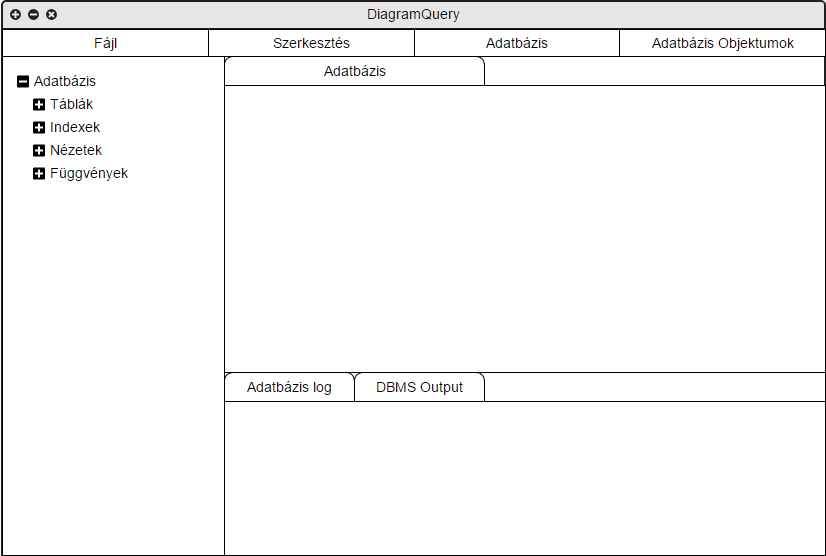
\includegraphics[scale=0.5]{mainWindow}
  \end{center}
 \caption{Fő ablak terve}
\end{figure}

A kapcsolódás után fogadja a felhasználókat a fő ablak, ami a 3.3-as ábrán látható. A legfontosabb, hogy rögtön munkához lehessen látni.
Érdemes úgy készíteni, hogy a képernyő nagy részét a szerkesztő tegye ki. Bal oldalon egy fában jelenjenek meg az adatbázis objektumai
(táblák, nézetek, függvények, indexek) és lehessen megtekinteni illetve törölni őket. A képernyőn jelenjen meg egy logban a futási idő,
illetve ha hiba történik, az legyen szemmel látható. PL/SQL szkriptek miatt érdemes egy külön lapon megjeleníteni a kiírt üzeneteket is.
Azonkívül legyen lehetőség a szerkesztő törlésére, mentésére, valamint már meglévő .sql kiterjesztésű fájl betöltésére is. A program adjon figyelmeztetést
törlés esetén. Mindemelett lehessen újra kapcsolódni az adatbázishoz arra az esetre, ha megszakadna a kapcsolat az adatbázissal, valamint
lehessen új kapcsolatot is nyitni, ami zárja be a jelenlegit. Legyen lehetőség az adatbázis objektumok megtekintésére és törlésére is.
A szerkesztőablakba beírt SQL lekérdezések, PL/SQL szkriptek, illetve egyedi parancsok (diagramok készítésére) hajtódjanak végre megfelelően,
és legyen látható pontosan mit hajtott végre a program. A szerkesztő betűtípusa legyen jól olvasható, a tabulátor mérete alapértelmezetten legyen
4, illetve az SQL és PL/SQL kulcsszavak legyenek kiemelve.
\newpage
\subsection{Komponensek}

\begin{figure}[ht]
  \begin{center}
  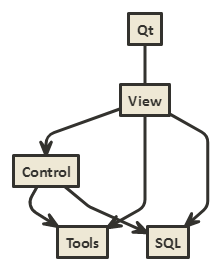
\includegraphics[scale=0.5]{components}
  \end{center}
 \caption{Komponensek}
\end{figure}

A program négy fő komponensből áll: Control, View, SQL, Tools. Mindegyik komponense a programnak külön felhasználható,
valamint bővíthető. Az SQL komponens azonban főként Oracle SQL-hez lett írva, így nem feltétlen működik minden
SQL variánsal, de ez később bővíthető. Az osztályokon kívűl egyéb függvényeket is tartalmaznak ezen komponensek, valamint
konstansokat is: ezek a jobb érthetőség és átláthatóság miatt kerültek a programba.

\subsubsection{Control}

\begin{figure}[ht]
  \begin{center}
  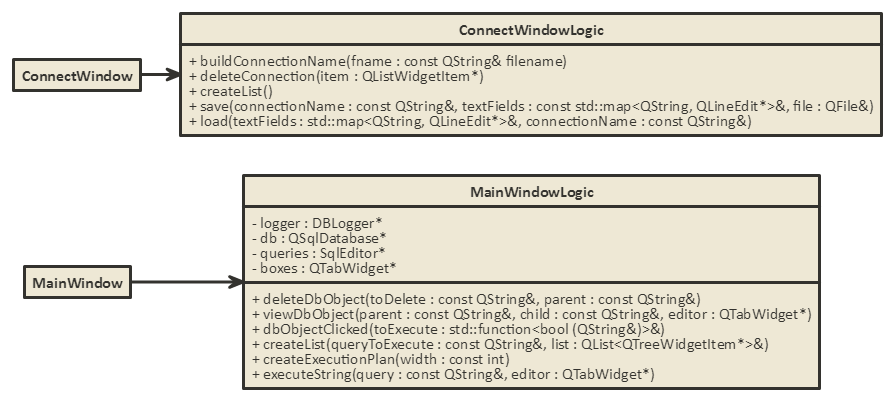
\includegraphics[max width=\textwidth]{control}
  \end{center}
 \caption{ Kapcsolódási- és főablak logikájának diagramja}
\end{figure}

Ebben a komponensben található a program logikája. Pontosabban itt, ebben a rétegben kerülnek a diagramok előállításra, valamint
itt kerülnek végrehajtásra a különböző lekérdezések. Miután a program végrehajtott egy utasítást, azután logolásra kerül a végrehajtás sikerettségét
jelző üzenet, valamint a hibaüzenet is sikertelen futás esetén.

\subsubsection{View}

\begin{figure}[ht]
  \begin{center}
  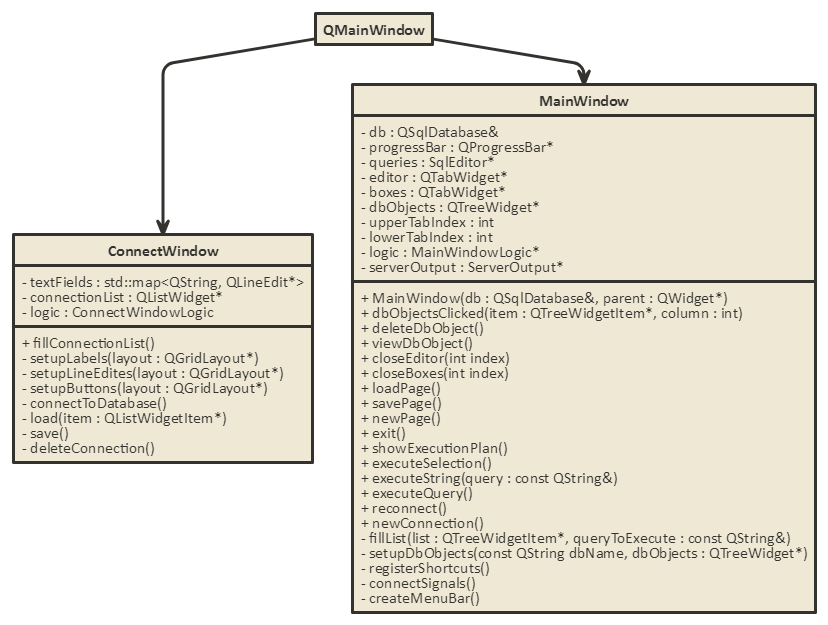
\includegraphics[max width=\textwidth]{view}
  \end{center}
 \caption{Kapcsolódási- és főablak diagramja}
\end{figure}

A View komponens felel a program kinézetéért. Itt van pontosan elrendezve minden nézetbeli elem, és itt vannak az események is lekezelve.
Fontos hogy jól érthető hibaüzeneteket jelenítsen meg ha valami nem rendeltetésszerűen történik, és ezt a felhasználó egyből észrevegye.
Későbbi szekcióban megtalálható a pontos terve a felhasználói felületnek, az alapján készítsük ezt el. A két legfontosabb függvény amit kiemelnék
a \textit{ConnectWindow::connectToDatabase()} és a \textit{MainWindow::reconnect()}.

ConnectWindow::connectToDatabase() metódus végzi el az adatbázishoz való kapcsolódást. Szüksége lesz az adatbázis, és a felhasználó adataira.
Az adatbázis adatai úgy mint a hoszt, port, serviceid (később esetlegesen a driver ami szükséges az adatbázishoz való kapcsolódáshoz). Valamint a 
felhasználó adatai úgy mint a neve és jelszava. A függvény írja ki ha hiba történik belépés során, illetve ha nem akkor csatlakozzon az adatbázishoz
és törölje a felhasználó jelszavát. Továbbá ez a metódus köti össze a kapcsolódási és főablakot.

A MainWindow::reconnect() metódus felelős a kapcsolat újboli kiépítésére. Bemenő adatai a felhasználó neve és jelszava. Abban az esetben ha a felhasználó
hibás adatokat ad meg, természetesen nem dobja el a régi kapcsolatot, hanem értesíti a felhasználót a hibáról. Megfelelő adatok esetén belépteti a felhasználót,
és folytathatja tovább eddigi munkáját. Erre legfőképp azért lehet szükség, mert bizonyos adatbázis szerverek (pl. Oracle) egy idő után kidobják a felhasználót.
Ilyenkor az egész programot újra kéne indítani ha erre nem adnánk lehetőséget.

\subsubsection{SQL}

\begin{figure}[ht]
  \begin{center}
  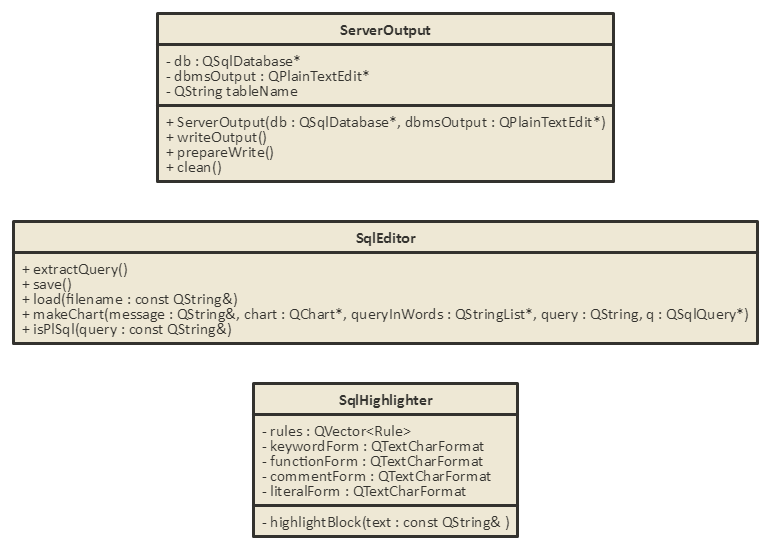
\includegraphics[max width=\textwidth]{sql}
  \end{center}
 \caption{SQL komponens osztályainak diagramja}
\end{figure}

Az SQL komponens végzi el a nyelvhez kapcsolódó feladatokat: szerkesztőfelülelet kialakítása, szintaxis kiemelése, a lekérdezések és szkriptek
megfelelő kiszedése. A cél az, hogy akár önmagában is használható legyen (feltéve, ha van egy adatbázis biztosítva hozzá), és minden SQL művelet
elvégezhető legyen a segítségével.

SQLHighlighter osztály reguláris nyelvtannal végzi el a kapott szöveg elemzését. Az összes SQL és PL/SQL kulcsszó\cite{sqlwords} kiemelését
elvégzi, továbbá a kommenteket, szám- és szövegliterálokat is másképp emeli ki a könnyebb érthetőség kedvéért.
Ennek az osztálynak egy metódusa van, a \textit{highlightBlock()} aminek a bemenete egy szövegliterál. Ezt a bemeneti szöveget elemzi a metódus,
majd reguláris kifejezések segítségével kiemeli a kulcsszavakat, és literálokat a szabályoknak megfelelően.

ServerOutput osztály a DBMS\_OUTPUT kiírására szolgál. Egy temporáris táblába tárolja el a kiírt sorokat amit a bufferből olvas, majd ezt kérésre
kiírja, és törli. Külön osztály azért szükséges ehhez, hogy kilépés esetén törölje maga után a létrehozott temporáris objektumokat a program a
RAII elvei szerint. Egyetlen fontos metódusa a \textit{writeOutput()}, aminek nincs bemenete és kimenete, csupán kiírja a megfelelő helyre a
buffer tartalmát.

Az SQLEditor osztály valósítja meg a fő szerkesztőfelületét az osztálynak. Ezen felül ez az osztály hozza létre a diagramokat, és kezeli le az
esetlegesen hibás bemeneteket. A szerkesztéssel kapcsolatos logika is itt található: itt történik a végrehajtandó utasítások kiemelése (persze a
végrehajtásuk nem ebben az osztályban történik), a diagramok feldolgozása és kirajzolása, valamint a lapok mentése és betöltése is. Annak érdekében
hogy jobban hasonlítson egy szerkesztőhöz, a jelenleg aktív sorokat is kiemeli, valamint ha futtatunk egy utasítást, vagy utasításokat, akkor azokat
is kiemeli hogy a felhasználó tisztában legyen azzal, hogy a program mit hajtott végre.

\subsubsection{Tools}

\begin{figure}
  \begin{center}
  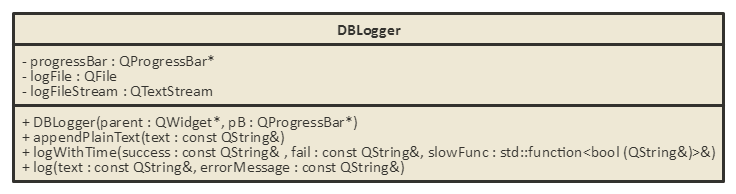
\includegraphics[max width=\textwidth]{tools}
  \end{center}
 \caption{Tools komponens osztályának diagramja}
\end{figure}

Ebben a komponensben a két osztályon felül egyéb eljárások illetve konstansok kerülnek eltárolásra.

A DBLogger osztály fontos szerepet játszik, mivel annak segítségével fogjuk a végrehajtandó utasításokat végrehajtani, és így lemérni a futás
idejüket. SQL lekérdezések készítésénél kritikus ennek a megléte, mivel így tudja a felhasználó javítani a lekérdezéseit szükség esetén.
\textit{DBLogger::logWithTime} metódusa fogja megoldani ezt, mégpedig egy függvény pointer segítségével. Szükséges bemenete a függvény amit
a programban kivánunk futtatni, és visszaad egy üzenetet arról hogy a művelet sikeres avagy sikertelen volt-e, valamint egy hibaüzenetet
sikertelen lefutás esetén.
\newpage
\section{Megvalósítás}

Ebben a szakaszban a konkrét megvalósítással foglalkozunk. Először a forrásfájlok fizikai elhelyezkedése kerül elő, majd az, hogy milyen eszközök
voltak használva a fejlesztés során, végül az egyes komponensekről, azon belül is a komponensekben található osztályokról lesz egy részletesebb leírás.

\subsection{Fájlok és könyvtárak fizikai elhelyezkedése}

A könyvtárak és forrásfájlok elhelyezkedése a következő:
\dirtree{%
.1 Control.
.2 ConnectWindowLogic.cpp.
.2 ConnectWindowLogic.h.
.2 MainWindowLogic.cpp.
.2 MainWindowLogic.h.
.1 Resources.
.2 favicon.png.
.1 SQL.
.2 ServerOutput.cpp.
.2 ServerOutput.h.
.2 SqlEditor.cpp.
.2 SqlEditor.h.
.2 SqlHighlighter.cpp.
.2 SqlHighlighter.h.
.1 Tools.
.2 Constants.h.
.2 DBLogger.cpp.
.2 DBLogger.h.
.2 GUITools.cpp.
.2 GUITools.h.
.1 View.
.2 ConnectWindow.cpp.
.2 ConnectWindow.h.
.2 MainWindow.cpp.
.2 MainWindow.h.
.1 main.cpp.
.1 QueryCreator.pro.
.1 resources.qrc.
}

\subsection{Eszközválasztás}

Egy olyan adatbázis-kezelő rendszer kellett, ami hatékony, mégis elérhető több operációs
rendszeren is, így lehet rá olyan klienst írni ami szinte bármilyen rendszeren elérhető.
A választás többek között ezért esett az Oracle SQL-re, hisz talán ez érhető ez a legtöbb
rendszerre, és figyelembe veszik a hatékonyságot a fejlesztés során.
Oracle SQL-hez több kezelő felület is elérhető, azonban a legjobban használható amit kiemelnék az az Oracle által készített SQL Developer, csakhogy ez a program Java
implementációjára hagyatkozik, így nem annyira hatékony. Ezért esett a választás a C++-ra, és a Qt keretrendszerre
hisz hatékonyak, és rengeteg funkcióval is rendelkeznek amik hasznosak lehetnek fejlesztés
során. Mivel Qt Creator szinte minden rendszeren elérhető amin a Qt is fordítható, így erre esett
a választás mint fejlesztő környezet, külön build keretrendszer nem lett használva.
Tesztelve manuálisan lett, így arra külön könyvtár nem került felhasználásra.

\subsection{Control}

\subsubsection{ConnectWindowLogic}

Ez az osztály felelős a kapcsolódási ablak logikájáért. Itt kerül előállításra a kapcsolat neve, valamint itt történik egy kapcsolat mentése, törlése, betöltése.

\begin{flushleft}
\textit{Metódusok}
\end{flushleft}
\textbf{createList()}: Elkészít egy QStringekből álló listát a Connection mappában lévő fájlokból, ezek tartalmazzák a kapcsolatok adatait. \\
\textbf{save}: Elmenti a kapcsolat adatait egy xml formátumú fájlba. \\
\textbf{load}: Betölti a kapcsolat adatait egy .xml kiterjesztésű fájlból. Mielőtt betöltené
törli az összes mező tartalmát arra az esetre, ha esetlegesen a felhasználó valamelyiket nem
töltötte volna ki kézzel. (Programmal való mentés esetén egy üres tag mindenképp lementésre
kerül.) \\
\textbf{buildConnectionName(QString\&)}: Felépíti a kapcsolat nevét, azaz az átadott QString nevével létrehoz egy
Connections/$<$string neve$>$.xml tartalmú QStringet majd visszaadja azt. A függvényben a QDir::separator() elválasztót
használjuk, így rendszerfüggetlen elválasztót kapva. \\
\textbf{deleteConnection(QListWidgetItem*)}: A fentebb említett buildConnectionName() metódus segítségével megépíti a kapcsolat nevét
ahhoz az elemhez amit paraméterként kap. Ha sikerül a törlés akkor törli az elemet is, és igazat ad vissza, különben hamisat.
Itt megemlíteném az elágazásban használt makrót: Q\_LIKELY. Qt saját makrója, ami segít a branch predictingben, így
hatékonyabb kódot generálhat. Érdemes megjegyezni, hogy jobb ennek a makrónak a használatát nem
túlzásba vinni, hisz sok hibás következtetés elég nagy teljesítménybeli romlást idézhet elő. A következő táblázatban részletesen
megtekinthető a késleltetési idő, például ha átrendezve az egész végrehajtandó kód már bekerül az instruction cachebe, akkor nyílván
gyorsabban végrehajtódik, mintha egy ugrás után kéne kiolvasni a memóriából.

Késleltetésre egy összehasonlító táblázat (Latency Numbers Every Programmer Should Know\cite{latency}) :
\begin{center}
\begin{tabular}{ l | c }
  L1 cache elérési ideje & 0.5 ns \\
  Rossz feltétel választása (branch mispredict) & 5 ns \\
  L2 cache elérési ideje & 7 ns \\
  Mutex zárás/nyitás & 25 ns \\
  RAM elérési ideje & 100 ns \\
  1 KB tömörítése Zippy-vel & 3 $\mu$s \\
  1 KB adat küldése 1 Gbps-es kapcsolaton keresztül & 10 $\mu$s \\
  4 KB véletlen adat olvasása SSD-ről & 150 $\mu$s \\ 
  1 MB olvasása szekvenciálisan a memóriából  & 250 $\mu$s \\
  Körút egy adatközpontban & 500 $\mu$s \\
  1 MB olvasása szekvenciálisan SSD-ről  &  1 ms \\
  Merevlemez olvasófejének mozgatása & 10 ms \\
  1 MB olvasása szekvenciálisan merevlemezről  &  20 ms \\
  Csomag küldése: CA$\rightarrow$Hollandia$\rightarrow$CA & 150 ms
\end{tabular}
\end{center}

\textbf{Megjegyzés:} 1 ms = 1 000 $\mu$s; 1 $\mu$s = 1 000 ns.

\subsubsection{MainWindowLogic}

Ez az osztály felelős a fő ablak logikájáért. Itt kerülnek előállításra a különböző modellek
amit továbbít a nézetnek az osztály, illetve ez az osztály készíti el a lekérdezési terveket is, és a lekérdezések végrehajtását is az osztály végzi.

\begin{flushleft}
\textit{Metódusok}
\end{flushleft}
\textbf{deleteDbObject(const QString\&, const QString\&)}: Törli az adatbázisból a paraméterként kapott objektumot (Tábla, Nézet, Index, Függvény). Egy egyszerű névtelen függvénnyel teszi ezt:

\begin{lstlisting}[language=C++]
  std::function<bool(QString&)> toExecute = [&](QString& failMessage)
\end{lstlisting}

Ez a standard könyvtárbeli típus egy függvény pointerre hasonlít, de pontosabban ez egy
függvény 'csomagoló' amibe bármilyen hívható objektum eltárolható. Használata egyszerűbb, kifejezőbb, és olvashatóbb mint az egyszerű függvény pointernek, egyetlen igazi hátránya
hogy kevésbé hatékony. Ez a fajta módszer van alkalmazva minden művelet mérésére, így a továbbiakban már nincs részletezve. \\
\textbf{viewDbObject(const QString\&, const QString\&, QTabWidget*)}: A paraméterként
kapott objektumról lekér információkat az adattáblából, majd megjeleníti azokat egy
QTableView-ban. A tábla oszlopait egyenlő mértékben felosztja az ablak méretéhez képest. \\
\textbf{dbObjectClicked(std::function$<$bool (QString\&)$>$\&)}: Lefuttatja a paraméterként
kapott függvényt. \\
\textbf{createList(const QString\&, QList$<$QTreeWidgetItem*$>$\&)}: elkészíti az adatbázis objektumok listáját. ForwardOnly tulajdonságát a lekérdezésnek igazra lehet állítani, hisz
sorrendben van szükség az adatokra, és így hatékonyabban működik. \\
\textbf{createExecutionPlan(const int)}: A kijelölt szöveghez, illetve ha nincs kijelölve a kurzorhoz legközelebb álló lekérdezéshez készít egy lekérdezési tervet, majd ezt betölti egy
QTreeWidget-be amit megjelenít. Megjelenítés után törli a lekérdezési tervet az adatbázisból. \\
\textbf{executeString(const QString\&, QTabWidget*)}: Ez a metódus hajtja végre a utasítást, amit paraméterként kapott. Ez lehet egy SQL lekérdezés, PL/SQL szkript, vagy egy diagram létrehozása. A diagram létrehozása nem itt történik, de ez az osztály logolja az utasítások végrehajtását.
\begin{flushleft}
\textit{Adattagok}
\end{flushleft}
\textbf{logger : DBLogger*} - ezen az adattagon keresztül kerülnek a függvények végrehajtásra, és kerülnek lemérésre. \\
\textbf{db : QSqlDatabase*} - ez az adatbázis objektumra mutató pointer, ezen keresztül hajtódnak végre az utasítások, illetve nyerhetők ki a hibák amik futás során keletkeznek. \\
\textbf{queries : SqlEditor*} - ezen pointeren keresztül lehet elérni azt az osztályt, amiben lekérdezésre kerül a feldolgozandó utasítás, illetve itt kerülnek előállításra a diagramok. \\
\textbf{boxes : QTabWidget*} - ezen adattag mögött található a fő ablakban is megtalálható
QTabWidget, amin van az adatbázis log, illetve a szerver kimenete.
\newpage
\subsection{SQL eszközök}

\subsubsection{ServerOutput}

Ez az osztály felelős azért, hogy lehetséges legyen a szerver kimenet megjelenítése a
programban.

\begin{flushleft}
\textit{Metódusok}
\end{flushleft}
\textbf{ServerOutput(QSqlDatabase*, QPlainTextEdit*)}: Az osztály konstruktora, egy random generátor segítségével készít egy nevet, amit elment a tableName adattagba, és ezen a néven fogja létrehozni a táblát az adatbázisban ami szükséges a kiíráshoz. Ezen felül engedélyezi a szerver kimenetet, a következő PL/SQL szkriptel:

\begin{lstlisting}[language=PL/I]
  BEGIN
    DBMS_OUTPUT.ENABLE (buffer_size => NULL);
  END;
\end{lstlisting}
\textbf{$\sim$ ServerOutput()}: Törli a kiíráshoz szükséges táblát, valamint felszabadítja a memóriát. \\
\textbf{writeOutput()}: Ez a metódus lekéri a bufferben lévő sorokat egy \textit{tableName} nevű adattáblába, majd lekéri őket, és utána törli a tábla tartalmát.

\begin{flushleft}
\textit{Adattagok}
\end{flushleft}
\textbf{db : QSqlDatabase*} - ez az adatbázis objektumra mutató pointer, ennek segítségével nyeri ki az osztály a szerver kimenet tartalmát. \\
\textbf{dbmsOutput : QPlainTextEdit*} - ez a fő ablakba lévő dobozra mutató pointer, ami kiírja a lekért sorokat. \\
\textbf{tableName : QString} - az ideiglenes tábla neve, amibe beilleszti majd kikéri a szerver bufferében lévő sorokat.

\subsubsection{SqlEditor}

Ez az osztály valósítja meg a fő ablakban található szerkesztőt. Itt készülnek el a diagramok, illetve itt szedi ki az utasításokat a szövegből.

\begin{flushleft}
\textit{Metódusok}
\end{flushleft}
\textbf{SqlEditor(QWidget*)}: Az osztály konstruktora, beállítja a betűtípust (Segoe UI, 11), illetve a
tabulátor méretét 4-esre. \\
\textbf{extractQuery()}: A lekérdezéseket szedi ki egy kurzor segítségével. Ha üres soron kerül meghívásra, akkor a sor előtti utasítás lesz végrehajtva. Ezek után RegExp segítségével
törli a kommenteket, illetve ha nem PL/SQL utasítás akkor a pontosvesszőt is, továbbá a felesleges whitespaceket, és per jelet. \\
\textbf{save()}: Elmenti a szerkesztő tartalmát egyszerű szövegként, .sql formátumban, operációs rendszer szerinti kódolásban. \\
\textbf{load(const QString\&)}: Betölti egy .sql formátumú fájl tartalmát, aminek kódolása
meg kell egyeznie az operációs rendszer alapértelmezett kódolásával. \\
\textbf{makeChart(QString\&, QtCharts::QChart*, QStringList*, QString, QSqlQuery*)}: Ez az osztály metódus a Qt Charts névteret használja, itt készül el a diagram. Mielőtt bármit lekérdezne elvégez néhány ellenőrzést hogy egyáltalán érdemes-e neki kezdeni a diagram készítésének, majd elkészíti a megfelelő diagramot. \\
\textbf{isPlSql(const QString\&)}: Néhány kulcsszó segítségével ellenőrzi hogy a paraméterként megadott utasítás PL/SQL utasítás-e: egyesével végigmegy a kulcsszavakon és megnézi hogy az utasítás valamelyikkel kezdődik-e, és ha igen igazat ad vissza, különben hamisat. A kulcsszavak az alábbiak: \textbf{DECLARE}, \textbf{BEGIN}, \textbf{CREATE OR REPLACE PROCEDURE}, \textbf{CREATE OR REPLACE FUNCTION}, \textbf{CREATE OR REPLACE PACKAGE}, \textbf{CREATE OR REPLACE TRIGGER}. \\
\textbf{highlightCurrentLine()}: ha kurzor helyzete megváltozik, akkor kiemeli az aktuális sort egy sárgás színnel.

\subsubsection{SqlHighlighter}

Ez az osztály végzi a szöveg szintaktikus kiemelését. A kulcsszavak az Oracle Dokumentációjából\cite{oracledocsref} lettek másolva. Egy két adattagot tartalmazó struktúra is megtalálható az osztályban, ami a kulcsszavak formázást egyszerűsíti.

\begin{flushleft}
\textit{Metódusok}
\end{flushleft}
\textbf{SqlHighlighter()}: A dokumentációban található kulcsszavakat és függvényeket kigyűjti és hozzáadja a \textbf{rules} vektorhoz, valamint a komment, és szövegliterálok reguláris kifejezését is. \\
\textbf{highlightBlock(const QString\& text)}: Ez a metódus végzi a szintaxis kiemelést. Valamint itt kerül beállításra a számliterálok alakja is, és környezettől függően máshogy lesz kiemelve, hisz például egy attribútum is tartalmazhat számot. \\
\begin{flushleft}
\textit{Adattagok}
\end{flushleft}
\textbf{rules : QVector$<$Rule$>$} - a szabályok alkotta vektor, ez tartalmazza a kulcsszavakat feldolgozó szabályokat, illetve a formázásukat. \\
\textbf{keywordForm : QTextCharFormat} - a kulcsszavak formázását leíró adattag (fekete színű, félkövér). \\
\textbf{functionForm : QTextCharFormat} - a függvények formáját leíró adattag (sötétkék színű, félkövér). \\
\textbf{commentForm : QTextCharFormat} - a kommentek-nek írja le a formázását ez az adattag (szürke színű). \\
\textbf{literalForm : QTextCharFormat} - a szám illetve szövegliterálok leírója (narancssárga színű).
\newpage
\subsection{Eszközök}
\subsubsection{DBLogger}

Ez az osztály végzi az utasítások mérését, és ha sikeresek/sikertelenek arról az üzenetet logolja a felhasználói felületen, illetve egy fájlba, ha azt sikeresen létre tudja hozni.

\begin{flushleft}
\textit{Metódusok}
\end{flushleft}
\textbf{DBLogger(QWidget*, QProgressBar*)}: Az osztály konstruktora, ez hozza létre a log fájlt is, ev\_honap\_nap.log formában. Ha nem létezne a Logs mappa, akkor azt létrehozza mielőtt megpróbálná a log fájlt megnyitni. \\
\textbf{appendPlainText(const QString\&)}: Kiír egy sort [$<$óra$>$:$<$perc$>$:$<$másodperc$>$] $<$üzenet$>$ formában a log fájlba, és az ablakba egyaránt. \\
\textbf{logWithTime(const QString\&, const QString\&, std::function$<$bool (QString\&)$>$\&)}: Átállítja a progressBar-t hogy jelezze egy függvény futása folyamatban, illetv lefuttatja a paraméterben kapott függvényt, valamint leméri ennek a futási idejét. Ha hiba nélkül lefutott a függvény, akkor kiírja a megfelelő üzenetet, valamint a futás idejét is, abban az esetben viszont ha nem sikerül, akkor csak az ezt jelző üzenet kerül logolásra. Futás után visszaadja hogy sikerült-e vagy sem megfelelően a függvény futása. \\
\textbf{log(const QString\&, const QString\&)}: Logolja a paraméterben kapott üzenetet, valamint ha a második paraméter nem üres QString, akkor azt is. A második paraméterben egy hibaüzenet kerül átadásra.

\begin{flushleft}
\textit{Adattagok}
\end{flushleft}
\textbf{progressBar : QProgressBar*} - folyamatjelző a fő ablakban. \\
\textbf{logFile : QFile} - ebben a fájlban található az aktuális log. \\
\textbf{logFileStream : QTextStream} - ebben a FileStream-ben van megnyitva az aktuális logfájl, abban az esetben ha meg lehetett nyitni.

\newpage
\subsection{Felhasználói felület}
\subsubsection{ConnectWindow}

Ez az osztály hozza létre a kapcsolódási ablakot. Itt lehet a kapcsolatokat kezelni, valamint itt lehet kapcsolódni az adatbázishoz, és ez az osztály nyitja meg a fő ablakot is, miután sikeresen létrehozza a kapcsolatot.

\begin{flushleft}
\textit{Metódusok}
\end{flushleft}
\textbf{ConnectWindow(QWidget*)}: Beállítja fixen, 800 x 170 méretre (pixelben) és letiltja az átméretezését az ablaknak. Az eseményeket is összekapcsolja: \textit{delete} billentyűre a deleteConnection() metódust, \textit{enter} billentyűre a connectToDatabase() metódust, és a dupla kattintásra a \textit{load} metódust. Ezeken kívűl meghívja a setup lezdetű metódusokat, hogy felépítse megfelelően a felületet. \\
\textbf{fillConnectionList()}: Törli a jelenlegi listát, és feltölti a kapcsolatok listáját a logic createList() metódusának segítségével. \\
\textbf{connectToDatabase()}: Kapcsolódik az adatbázishoz az OCI driver segítségével. A mezőket kinyeri a textfieldsből (host, service, port, username, password), majd megpróbál kapcsolódni az adatbázishoz. Siker esetén törli a jelszót a memóriából, létrehozza a fő ablakot, majd eltűnteti és törli a kapcsolódási ablakot a memóriából. \\
\textbf{load(QListWidgetItem*)}: Ez a metódus csupán meghívja a logika load() metódusát textFields-el, és a paraméterben kapott item-el. \\
\textbf{save()}: Megkísérli a kapcsolat adatainak elmentését. Az adatokat nem ellenőrzi külön, hisz például portnál se lehet szöveget csak számot megírni, aminek ellenőrzését elvégzi a felhasználói felület egy validátor segítségével. Hiba esetén (nem lehet menteni mert létezik ilyen kapcsolat, vagy nem lehet létrehozni a könyvtárat) a program hibát dob, és leáll a működése. \\
\textbf{deleteConnection()}: Törli a kijelölt kapcsolatot, és sikertelen törlés esetén kiír egy hibaüzenetet. \\
\textbf{setupLabels(QGridLayout*)}: Létrehozza a címkéket az ablakhoz, és hozzáadja ahhoz őket. \\
\textbf{setupLineEdites(QGridLayout*)}: Létrehozza a mezőket az ablakhoz, hozzáadja a textFields-hez őket, valamint a port mezőhöz beállít egy validátort, így csak 0 és 10000 közti számot lehet megadni portként. \\
\textbf{setupButtons(QGridLayout*)}: Létrehozza a gombokat az ablakhoz, valamint beállítja az eseményeket is, \textbf{kapcsolódás} gombra kattintva meghívja a connectToDatabase() metódust, míg \textbf{mentés} gombra kattintva meghívja a save() metódust.

\begin{flushleft}
\textit{Adattagok}
\end{flushleft}
\textbf{textFields : std::map$<$QString, QLineEdit*$>$} - ez az adattag tartalmazza az ablakban lévő mezőket, ezen keresztül lehet később hivatkozni rájuk, és szerkeszteni őket. \\
\textbf{connectionList : QListWidget*} - egy listában jeleníti meg a kapcsolatokat, itt lehet törölni és betölteni őket később. \\
\textbf{logic : ConnectWindowLogic} - az ablak logikáját tartalmazza, ennek részletezése korábban megtörtént a Control nevű szakaszban.

\subsubsection{MainWindow}

A főablakot valósítja meg, a 3.3-as ábrán látható terv alapján. Itt történik minden művelet a kapcsolódás után.

\begin{flushleft}
\textit{Metódusok}
\end{flushleft}
\textbf{MainWindow(QWidget*)}: Az ős osztályból öröklődött konstruktor, itt nincs szükség rá, így törlése kerül. \\
\textbf{MainWindow(QSqlDatabase\&, QWidget*)}: Alapértelmezetten 1024x768 pixelben létrehoz egy ablakot és középre helyezi, azonban kis képernyő esetén kissebb méretben jeleníti azt meg. A segédmetódusok segítségével létrehozza az ablak elemeit, és beállítja az eseménykezelőt is. \\
\textbf{dbObjectsClicked(QTreeWidgetItem*, int)}: Ez kezeli le azt az eseményt, ha egy adatbázis objektumra kattintanak, és meghívja a megfelelő toFill metódust egy függvény pointer segítségével.
\begin{lstlisting}[language=C++]
bool (MainWindow::*toFill) (QTreeWidgetItem*);
\end{lstlisting}
Ennek a típusnak a magyarázata: MainWindow osztálybeli metódusra mutató, toFill nevű függvény pointer, aminek metódusa egy darab QTreeWidgetItem* paramétert vár. Értékadás a következőképp történik például:
\begin{lstlisting}[language=C++]
toFill = &MainWindow::fillFunctionList;
\end{lstlisting}
Bizonyos fordítók esetén az osztálynév elhagyása nélkül is működik osztályon belül, azonban ez a standard verzió, így érdemes ezt használni, mivel garantáltan csak így működik. Továbbá a függvény meghívása a következőképp történik:
\begin{lstlisting}[language=C++]
(this->*toFill)(item)
\end{lstlisting}
\textbf{deleteDbObject()}: Megerősítést kér a felhasználótól, majd a logic deleteDbObject() metódusával törli az adatbázis objektumot. \\
\textbf{viewDbObject()}: Lekéri a jelenleg kijelölt adatbázis elemnek a nevét, és hogy ha az nem egy fő elem (Tábla, Nézet...) akkor a logic viewDbObject() metódusának segítségével lekéri annak az adatait. Az ellenőrzésre az elején hogy van-e kijelölt elem azért van szükség, mert menüből is elérhető ez a funkció. \\
\textbf{closeEditor(int)}: Bezárja a felső dobozban található lapot, amelyiknek a számát paraméterben kapta. Azonban ha ez a szám 1, akkor nem csinál semmit, hisz a szerkesztőablak nem zárható be. \\
\textbf{closeBoxes(int)}: Bezárja az alsó dobozban található lapot, amelyiknek a számát paraméterben kapta. Azonban ha ez a szám 2-nél kissebb, akkor nem csinál semmit, hisz a Logoló és a szerver kimenetét kiíró lap nem zárható be. \\
\textbf{loadPage()}: Betölti egy sql formátumú fájl tartalmát a szerkesztőablakba. Ennek a betöltését az SQLEditor végzi. \\
\textbf{savePage()}: Elmenti a szerkesztőfelület tartalmát egy .sql formátumú fájlba, ezt is az SQLEditor osztály végzi. \\
\textbf{newPage()}: Megerősítés után törli a szerkesztőfelület tartalmát. \\
\textbf{exit()}: Megerősítés után bontja a kapcsolatot és kilép a programból. \\
\textbf{showExecutionPlan()}: Logic createExecutionPlan() metódusát meghívva létrehoz egy lekérdezési tervet, és ha ez sikeres, akkor betölti azt az alsó dobozba. \\
\textbf{executeSelection()}: A kijelölt szöveget betölti egy változóba, törli belőle a felesleges whitespaceket és pontosvesszőt, majd ezek után megkísérli végrehajtani azt. \\
\textbf{executeString(const QString\&)}: felkészíti a szerver kimenetet arra az esetre hogy ha szükséges lenne a kiírása, majd futtatja a paraméterként kapott QString-et, végül eltakarít maga után. \\
\textbf{executeQuery()}: meghívja az executeString metódust a queries extractQuery() metódusával kinyert QString-re. \\
\textbf{reconnect()}: Megpróbál újrakapcsolódni az adatbázishoz. Bekéri a felhasználónevet (amit automatikusan kitölt alapból) és jelszót, majd megkísérel újracsatlakozni. Hiányzó vagy hibás mező esetén hibát ad, ha sikeres a kapcsolódás akkor kiírja hogy sikeresen újrakapcsolódott. \\
\textbf{newConnection()}: Megerősítés után bontja a kapcsolatot, és nyit egy új kapcsolódási ablakot. \\
\textbf{setupDbObjects(const QString, QTreeWidget*)}: a bal oldali fát felépíti, és beállítja a fa fő címkéjét. \\
\textbf{registerShortcuts()}: beállítja a felhasználói dokumentációba részletezett billentyűkombinációkat. \\
\textbf{connectSignals()}: beállítja a következő eseményeket: duplakattintás hatására dbObjectClicked kerül meghívásra, illetve a tabok bezására beállítja rendre a closeEditor(), closeBoxes() metódusokat. \\
\textbf{createMenuBar()}: elkészíti a felület tervében megadott menüt. \\
\textbf{fillList(QTreeWidgetItem*, const QString\&)}: feltölti a kattintot adatbázis objektumok listáját. \\
\textbf{fillTableList(QTreeWidgetItem*)}: feltölti a táblák listáját. \\
\textbf{fillIndexList(QTreeWidgetItem*)}: feltölti az indexek listáját. \\
\textbf{fillViewList(QTreeWidgetItem*)}: feltölti a nézetek listáját. \\
\textbf{fillFunctionList(QTreeWidgetItem*)}: feltölti a függvények listáját.
\begin{flushleft}
\textit{Adattagok}
\end{flushleft}
\textbf{db : QSqlDatabase\&} - egy adatbázis objektumot tárol, ezen kerülnek végrehajtásra a lekérdezések. \\
\textbf{progressBar : QProgressBar*} - folyamatjelző hosszú utasítások esetére. \\
\textbf{queries : SqlEditor*} - a szerkesztőablakot ezen keresztül lehet elérni. \\
\textbf{editor : QTabWidget*} - a felső doboz az ablakban, amin alapértelmezetten a queries van tárolva. \\
\textbf{boxes : QTabWidget*} - az alsó doboz az ablakban, amin két lap található alapértelmezetten: az adatbázis log, és a szerver kimenet. \\
\textbf{dbObjects : QTreeWidget*} - a bal oldali QTreeWidget, ebben találhatóak meg az adatbázis objektumok nevei, illetve itt kezelhetőek azok. \\
\textbf{upperTabIndex : int} - az éppen aktív tab indexe a queries-ben. \\
\textbf{lowerTabIndex : int} - az éppen aktív tab indexe az editor-ban. \\
\textbf{logic : MainWindowLogic*} - az ablak logikája, korábbi szakaszban részletezve van a pontos funkcionalitása. \\
\textbf{serverOutput : ServerOutput*} - a szerver kimenetét lehet ezen az objektumon keresztül kezelni.

\section{Továbbfejlesztési lehetőségek}

Ha több különböző adatbázis driverek használata elérhetővé válna, akkor több lehetőség nyílna meg a felhasználó számára, erre a Qt megfelelő felületet biztosít. A Qt keretrendszer natívan támogatja az alábbi adatbázis-kezelő rendszereket: IBM DB2 (7.1+), Borland InterBase, MySQL, Microsoft SQL Server,	PostgreSQL (7.3+),	SQLite 2,	SQLite 3,	SQLite 3 Symbianhoz, Sybase Adaptive Server (Qt 4.7 óta elavult). Mindegyiknek megvan a maga előnye, például a MySQL nyílt forráskodú, így jobban belefolyhat a fejlesztésébe is akár aki használni akarja. Ezeknek, és további relációs adatbázisoknak az összehasonlítását megtekintheti a Wikipédián\cite{rdbmscompare}.

Továbbá a felhasználói felületeten is javítanának az alábbi változtatások: ha gyakori eset, hogy a felhasználók szerkeszteni akarják a kapcsolatot akkor egy extra gombot lehetne a felületre helyezni. Az előbbi fejlésztés bevezetése után a kapcsolódási ablaknál kellene egy extra lehetőség az adatbázis driver típusának kiválasztására is.

A fő ablakon is van hely a fejlesztésre: a szerkesztő ha számozva lenne akkor könnyebben hivatkozhatna illetve kereshetne a felhasználó egy-egy sort, illetve az elválasztó helyének elmentése kilépéskor (esetleg külön felületen való beállítását) hasznos kényelmi szempontból, illetve összességében a szerkesztőfelület testreszabása nagyban javítana a felhasználói élmményen (betűtípus, tab mérete, ...). Ezen felül a tabokat leválasztása is hasznos lenne: átláthatóbbá tenné a felületet.

A diagramoknál több típus sincs implementálva, ezek szintén hasznosak lehetne, és a jelenlegieket is bővíteni lehetne új opciókkal, így szélesebb választékot adva. Azonkívűl mentés lehetősége nagyban javítana a programot: így fel lehetne használni a diagramokat prezentációhoz, kinyomtatni őket, vagy egy honlapra felrakni.

Utoljára, de nem utolsó sorban nagyban javítana a programon a többszálusítás, így robosztusabb lenne, és könnyebben megszakíthatóvá válnának az egyes műveletek.

\section{Tesztelés}

A QueryCreator-ban amely funkciókat lehetne egység tesztekkel ellenőrizni, azok főleg a Qt könyvtárban már tesztelve lettek, részletes dokumentáció van írva hozzájuk ami alapján könnyű őket használni. Ezért is a programot inkább a grafikus felületen teszteltem, hogy tényleg minden megfelelő-e, és hogy nem keletkezik semmilyen hiba.

\subsection{Kapcsolódási ablak}
Fontos szempont, hogyha véletlen rákattintana a felhasználó a kapcsolódásra, vagy entert nyomna, akkor ne szálljon el a program: ekkor egy hibaüzenetet jelenít meg a sikertelen kapcsolat létrehozáskor. A mezőknél bármilyen hosszú, illetve rövid (üres) szöveget adunk meg, akkor működjön megfelelően a program, továbbá portnak csak egy 0 és 10000 közötti számot lehessen megadni. Kapcsolat betöltése esetén ne maradjon meg régi érték, és hibás adatot ne töltsön be. Azaz ha azt adjuk meg portnak egy fájlban hogy almafa, akkor ne töltse be, illetve csak a megfelelő tagekkel törődjön. Mindez tesztelve lett, és az elvárásoknak megfelelően működik.

Mentés esetén fontos hogy ne szálljon el a program ha olyan nevet adunk meg amit nem lehet az operációs rendszer sajátosságai miatt létrehozni, ilyen lehet Windows esetén a kérdőjel, a kettőspont, és még néhány karakter. Ezen felül ha megpróbálunk létrehozni egy kapcsolatot létező névvel, akkor erre figyelmeztessen a program, és üres néven ne lehessen menteni. Ezen szempontoknak eleget tesz a program, és tesztelve lett.

Kapcsolatok törlésénél felmerülhet mint hiba hogy a felhasználónak nincs joga hozzá, illetve hogy már törölve lett a fájl. Ha ez történne, arról kap a felhasználó egy figyelmeztetést. Illetve megerősítést vár a program törlés előtt, így nem kerül egy kapcsolat se véletlenül törlésre.

\subsection{Fő ablak}

A bal oldalon lévő adatbázis objektumoknál azt teszteltem, hogy ha nem egy objektum, hanem csak egy címke van kijelölve, akkor ne történjen semmi törlésnél, illetve megtekintésnél. Adatbázis objektumnál viszont legyen figyelmeztetés törlés esetén, ez megfelelően működik.

A program fő részére, azaz a szerkesztőablakra külön tesztesetek találhatóak a lemezen:
\begin{itemize}
  \item \textbf{Test01\_SQL.sql} nevű fájl az alapvető SQL lekérdezéseket tartalmazza. Ez főleg azt teszteli, hogy a lekérdezések megfelelően vannak-e kiszedve a szövegből.
  \item \textbf{Test02\_PLSQL.sql} fájl a szerver kimenetét teszteli.
  \item \textbf{Test03\_DiagramTest.sql} a diagramokat teszteli, hogy a dokumentációban megadott megkötéseket teljesítik-e. Minden hibás lekérdezést lefed, illetve azt, hogy helyesen
  jelennek meg-e.
  \item \textbf{Test04\_ExplPlan.sql} a lekérdezési tervet teszteli, hogy megfelelően elkészül-e, illetve nem megfelelő lekérdezés esetén hibát ad-e a felhasználónak.
  \item \textbf{Test05\_DiagramTest2.sql} a diagramokat teszteli, hogy megfelelő input esetén az elvárt diagram jelenik-e meg.
\end{itemize}

Ezen tesztek futtatása során derült fény arra a hibára, hogy újracsatlakozás után nem működik a szerver kimenete. Mivel a konstruktorban lett a szerver kimenete engedélyezve, így nyílvánvalóan újrakapcsolódás esetén ez nem futott le újból, ezért nem működött a kiírás. Ezen felül kiderült az is, hogy a diagramkészítő nem megfelelő hibát ad vissza minden esetben, így ez is javítva lett.